%----------------------------------------------------------------------------
\chapter{Overview of local search-based pattern matching}
%----------------------------------------------------------------------------
\label{chap:overview}


Probably the biggest drawback of the \eiq framework is the memory consumption of its incremental algorithm. In order to overcome this limitation, we adapted a model sensitive local search-based pattern matching algorithm described in \cite{DBLP:journals/sosym/VarroDWS15}. This algorithm has a much smaller memory footprint, as well as the initial pattern matching execution takes also less time compared to the Rete incremental approaches.


\section{Related work}
\label{sec:relatedwork}

There are several modeling tools that implement pattern matching in addition to \eiq, such as ATL, Eclipse OCL, FUJABA, FunnyQT, and GrGen.NET. 

\emph{ATL}~\cite{DBLP:conf/uml/JouaultK05} defines a hybrid, textual language for defining graph transformations. It is called hybrid, for it has declarative language elements, but in order to ease formulation of complex rules, imperative instructions can also be used. ATL uses local search-based pattern matching, but applies different heuristics to determine the order of search operations. As it was described in~\cite{DBLP:conf/models/TisiPC13}, a parallel algorithm provides the matchings. %Also, the ATL has support for execution over various modeling domains, like...

\emph{Eclipse OCL}~\cite{eclipse:ocl} supports the declarative definition, and evaluation of OCL~\cite{OCL:Spec} constraints over EMF models. In this case, despite the declarative description of the pattern, the OCL constraint encodes the execution order of search steps to find elements that conform all constraints of the description. Also, Eclipse OCL has incremental evaluation support~\cite{DBLP:journals/jss/CabotT09}.

%\emph{FUJABA}~\cite{DBLP:conf/icse/NickelNZ00} provides a graphical language for specifying model transformation rules, and relies on local search-based pattern matching. It uses a breadth-first traversal of \emph{search graphs} with edge weights based on the multiplicity of references, as opposed to our adapted model-sensivive, dynamic programming based search plan calculation.

\emph{FUJABA}~\cite{DBLP:conf/icse/NickelNZ00} provides a graphical language for specifying model transformation rules, and relies on local search-based pattern matching. It uses \emph{story diagrams} for the execution~\cite{DBLP:journals/eceasst/GieseHS09}, and applies a dynamic strategy concerning the traversal of the instance model. This means for every object, the following step is made in the direction of the reference with the lowest multiplicity. The execution times presented in~\cite{DBLP:journals/eceasst/GieseHS09} are very promising regarding this approach. We can say that \emph{SDMLib} is the successor of FUJABA, which won the best performance award on the Transformation Tool Contest 2014~\cite{DBLP:conf/staf/EickhoffGLZ14} by generating Java code for search execution.

\emph{FunnyQT} is a Clojure library supplying a comprehensive set
of model querying and transformation services to the user~\cite{DBLP:conf/gg/Horn15}. According to~\cite{DBLP:conf/icmt/Horn13}, it supports pattern matching using an internal DSL implemented with Clojure’s metaprogramming facilities. The constraint evaluation order is defined by the user. 

\emph{GrGen.NET}~\cite{DBLP:conf/agtive/BatzKG07} also implements pattern matching based on local search philosophy. It calculates search plans based on a cost model, that estimates a \emph{backtracking} and an \emph{execution time} for an operation. The used search plan has the lowest total cost of operations possible. 

The algorithm we introduce in this work uses a search plan calculation algorithm that differs from the ones mentioned above. Also, the \eiq framework is unique in a way that the declaratively defined patterns can be executed using any of the local search or the incremental algorithm, without specifying the concrete steps of the execution.


\section{Algorithm adaptation}
\label{sec:algorithm-adaptation}
%TODO adaptation description?

In order to efficiently integrate the local search-based algorithm, we were required to adapt many existing components of the \eiq framework, more specifically parts of the \emph{pattern matcher engine}. The architecture overview of the engine is depicted in \autoref{fig:overview_core}:

\begin{enumerate}
	\item \emph{\baseindex} collects the instances of \texttt{EClasses}, \texttt{EReferences} and \texttt{EDataTypes} contained in a model,
	\item the \emph{Pattern definition} holds the query that is to be evaluated over the instance model, 
	\item the \emph{Pattern matcher} uses the pattern matcher algorithm to generate the result based on the \eiq Base Index and the Pattern definition, and
	\item the \emph{Match set} contains the result tuples.
\end{enumerate} 

\begin{figure}[!htp]
	\centering
	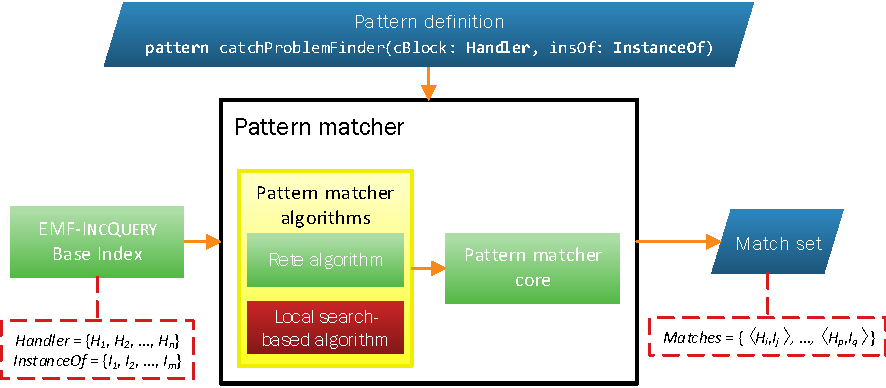
\includegraphics[width=\textwidth]{figures/pdfs/overview_core.pdf}
	\caption{The pattern matcher engine of \eiq}
	\label{fig:overview_core}
\end{figure}

In the introductory example, the base index would provide sets filled with the instances of the elements found in the metamodel, such as \texttt{Handler} and \texttt{InstanceOf}, as indicated in the lower left corner of \autoref{fig:overview_core}. The \catchproblem pattern definition states that the expected matches are supposed to be tuples with type $\langle \mathtt{Handler, InstanceOf}\rangle$, as illustrated below the match set in the diagram.

Our contribution to the engine (emphasized with solid red background) is the \emph{local search-based algorithm}, at least in the extent of this thesis. Prior to the implementation, we solved several adaptation issues.  A typical task was to decide how to extend already existing interfaces in order to obtain all the information needed for executing the algorithm. One of the main design guidelines was generalization of the existing solution, so that several pattern matching algorithms may coexist in the \eiq framework.

In as a result of our work, we proposed a common interface for pattern matching algorithms. In addition, using the chosen solution, users can select the appropriate algorithm runtime, according to their needs. We also prepared the pattern matcher runtime for parallel search execution, for the computation of matches can be done by multiple threads simultaneously. The details about search execution is in \autoref{sec:search-execution}.

While the \emph{Graph pattern matcher engine} provides the basic functions of \eiq, there are many accompanying tools to ease the use of the provided features. To introduce the layered architecture of the toolkit based on \cite{DBLP:journals/scp/UjhelyiBHHIRSV15}, a diagram of its structure is shown in \autoref{fig:overview}. 

\begin{figure}[!htp]
	\centering
	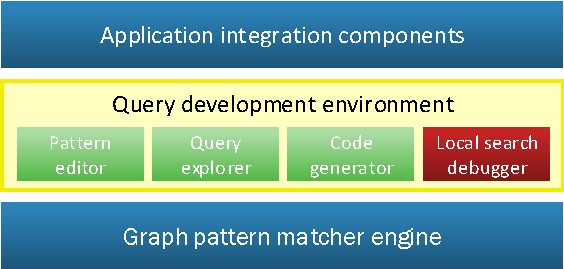
\includegraphics[width=0.7\textwidth]{figures/pdfs/overview}
	\caption{The architecture of \eiq}
	\label{fig:overview}
\end{figure}

The \emph{Query development environment} (QDE) provides tooling related to defining and debugging queries. One of the major components is the (i) \emph{Pattern editor}. This is an Xtext-based \cite{Xtext} editor for IQPL with syntax highlighting, auto-completion support and pattern well-formedness validation. The purpose of the (ii) \emph{Query explorer} is to evaluate complex queries on selected EMF models, and to visualize the match set of each pattern. Another very important part of the QDE is the (iii) \emph{Code generator}. It is tightly connected to the editor, as well as registered into the Eclipse builder framework. Thanks to this strong coupling with the IDE, code generation is executed after pattern definitions are modified, and saved. The output of the generation process is a pattern-specific Java code, that helps the integration of \eiq to Java applications by creating type-safe API for matchers. 

To further extend the capabilities of the QDE, we developed a (iv) \emph{Local search debugger} (highlighted with solid red background in the overview). It is designed to help the pattern developers understand and debug the local search-based pattern matching process by providing a visual representation of the calculated search plan, and to support step-by-step execution capability. \autoref{sec:lsdebugger} introduces the new debugger component and its capabilities in detail.


\eiq provides several application integration components as well, as indicated in the top part of \autoref{fig:overview}. They are not discussed in this work in detail, but they provide an API for accessing the features of the \eiq framework from Java programs.


\section{Pattern matching workflow}
\label{sec:pattern-matching-workflow}

We separate the local search-based pattern matching tasks into two categories. The first category is \emph{design time} tasks, and the second is \emph{execution time} tasks. Our pattern matching workflow is depicted in \autoref{fig:workflow}.

\begin{figure}[!htp]
	\centering
	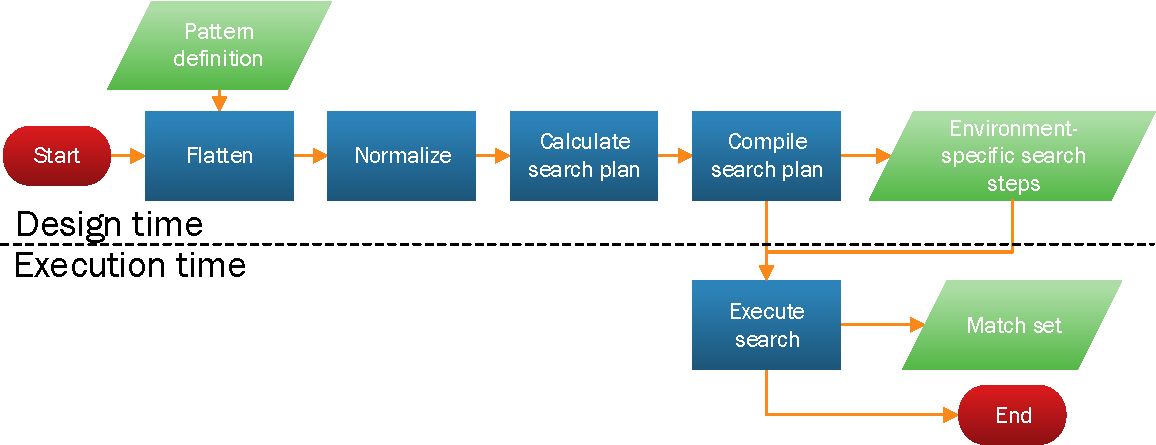
\includegraphics[width=\textwidth]{figures/pdfs/query_execution_workflow.pdf}
	\caption{The local search-based pattern matching workflow}
	\label{fig:workflow}
\end{figure}

The majority of the steps of the workflow are considered to be \emph{design time} tasks. The first task is to \emph{flatten} the input \emph{pattern description}. The pattern description may refer to other patterns, and flattening means the resolution of these references. As a result, a \emph{flat pattern} is created that unifies all constraints and variables, both from the referrer and the referee patterns. This allows to optimize on a global scale, rather than locally for patterns. It is important to add that semantics of the pattern is preserved throughout the process. Details about the implemented flattener algorithm is discussed in \autoref{sec:flattening}.

In the next step the flattened pattern is \emph{normalized}. This means an analysis in order to remove redundant, thus unnecessary constraints. For instance, type checking multiple times for the same variable, and with the same type is omitted. This step also unifies variables among equalities.

From the normalized pattern the \emph{local search planner} calculates a \emph{search plan} in the third step of the above workflow. In this case, this means an ordering of the constraints contained in the pattern. At this point all constraints and variables are directly contained in a normalized, flattened pattern that provides a global search space for the search plan calculation. As it was already mentioned in \autoref{sec:patternlanguage}, the declarative definition of patterns using IQPL does not hold information about the order of constraint enforcement and computation of the matches of a pattern. This requires the local search planner component to create the search operation sequence that finds substitutions for variables. This list of search operation is derived from an ordered list of constraints, which is done in \emph{compile search plan} step. The outcome of design time tasks is a list of \emph{environment-specific search steps}. In case of EMF, these environment specific search operations heavily rely on the efficient EMF reflective API, which is introduced in \autoref{sec:emf-reflection}, to obtain possible substitutions for the variables.

During \emph{execution time}, this list of search steps determines the order of variable substitutions. In the \emph{execute search} phase, the executor looks for substitutions that satisfy all constraints of the pattern. In the current application, it means that at some point, each variable is assigned a model element to check if it satisfies the description of the pattern. The details of search plan execution is detailed later in \autoref{sec:search-execution}.

To demonstrate the effects of the tasks depicted in \autoref{fig:workflow}, the flattened version of the \catchproblem pattern is presented in \autoref{lst:catch_flat} under the name \mbox{\texttt{catchProblemFinder\_flattened}}. 

% This prevents the listing to be split between pages
\begin{figure}[!htbp]
\listingiqpl{catch_flat}{Flattened pattern} 
\end{figure}

The body has all constraints from both \catchproblem and \handlervar, as well as additional equalities that declare the variables used to serve as parameters for the pattern call constraint, and the corresponding variables from the flattened pattern are equal. New variables coming from the flattening process are prefixed with "\handlervar\_".


A normalized version of the \mbox{\texttt{catchProblemFinder\_flattened}} pattern is \mbox{\texttt{catchProblemFinder\_flattened\_normalized}} (contained in \autoref{lst:catch_flat_normalized}). To achieve better readability of the created pattern description, we unified the variables with longer names into variables with shorter names along equalities, and also simplified the name of \texttt{handlervar\_param} to \texttt{param}.  

% This prevents the listing to be split between pages
\begin{figure}[!htbp]
	\listingiqpl{catch_flat_normalized}{Normalized pattern} 
\end{figure}

From the flattened and normalized pattern description, the search plan depicted in \autoref{tab:flat-norm} can be obtained. The details of the search plan calculation is included in \autoref{sec:localsearch}

\begin{table}[h]
	\centering
	\begin{tabular}{c|l}
		\hline
		& Constraint \\ \hline
		1: & \texttt{varRef} is of type \texttt{Identifier} \\
		2: & \texttt{varRef} is in \texttt{operand} relation with \texttt{insOf} \\
		3: & \texttt{insOf} is of type \texttt{InstanceOf} \\
		4: & \texttt{varRef} is in \texttt{param} relation with \texttt{refersTo} \\
		5: & \texttt{param} is referenced by \texttt{cBlock} in \texttt{parameter} \\
		6: & \texttt{cBlock} is of type \texttt{Handler} \\
		
	\end{tabular}
	\caption{Search plan for the flattened pattern}
	\label{tab:flat-norm}
\end{table}

If we compile the search plan for our introductory EMF-based example as the final step of the design time tasks, the list of environment specific search operations will be the following:
\begin{enumerate}
	\item Collect all instances that are of type \texttt{Identifier}. Then, one-by-one substitute the values to variable \texttt{varRef} and advance to the next search operation.
	\item For the current value of \texttt{varRef}, enumerate all values which can navigate to it on an \texttt{operand} reference. Substitute each enumerated element to \texttt{insOf}, then go on to the next operation.
	\item Check if the type of the substituted element for variable \texttt{insOf} is \texttt{InstanceOf}.
	\item Get all elements reachable from \texttt{varRef} by navigating on the \texttt{param}  relation. Substitute each element reached this way in place of variable \texttt{refersTo}, then advance to the next operation.
	\item Collect all elements that have the value of \texttt{param} in their \texttt{parameter} relation, then substitute each to \texttt{cBlock}.
	\item Check if \texttt{cBlock} has a substituted element of type \texttt{Handler}.
\end{enumerate}

This step is then followed by the \emph{execution task} on the given instance model. During the execution in this current minimal example, there are only a few elements in every steps that should be considered. There is only one match in this case, a tuple that is $ \langle \mathtt{hdl}, \mathtt{io} \rangle$ (using the notation of the hand drawn instance model in \autoref{fig:example-instancemodel-handdrawn}).
